\documentclass[11pt]{article}
\usepackage{geometry}                
\geometry{letterpaper}                   

\usepackage{graphicx}
\usepackage{amssymb}
\usepackage{epstopdf}
\usepackage{natbib}
\usepackage{amssymb, amsmath}
\usepackage{pdfpages}
\DeclareGraphicsRule{.tif}{png}{.png}{`convert #1 `dirname #1`/`basename #1 .tif`.png}

%\title{Title}
%\author{Name 1, Name 2}
%\date{date} 

\begin{document}



\thispagestyle{empty}

\begin{center}
\includegraphics[width=5cm]{ETHlogo.eps}

\bigskip


\bigskip


\bigskip


\LARGE{ 	Lecture with Computer Exercises:\\ }
\LARGE{ Modelling and Simulating Social Systems with MATLAB\\}

\bigskip

\bigskip

\small{Project Report}\\

\bigskip

\bigskip

\bigskip

\bigskip


\begin{tabular}{|c|}
\hline
\\
\textbf{\LARGE{Spread of news in a random network of agents}}\\
%\textbf{\LARGE{...}}\\
\\
\hline
\end{tabular}
\bigskip

\bigskip

\bigskip

\LARGE{Blum Josef, Kazakov Dmitry,
	
	Machacek David, Martin Kevin}



\bigskip

\bigskip

\bigskip

\bigskip

\bigskip

\bigskip

\bigskip

\bigskip

Zurich\\
Dec 2017\\

\end{center}



\newpage

%%%%%%%%%%%%%%%%%%%%%%%%%%%%%%%%%%%%%%%%%%%%%%%%%

\newpage
\section*{Agreement for free-download}
\bigskip


\bigskip


\large We hereby agree to make our source code for this project freely available for download from the web pages of the SOMS chair. Furthermore, we assure that all source code is written by ourselves or cited correctly and is not violating any copyright restrictions.

%\begin{center}

\bigskip


\bigskip


%\begin{tabular}{@{}p{3.3cm}@{}p{6cm}@{}@{}p{6cm}@{}}
%\begin{minipage}{0.5cm}

%\end{minipage}

\begin{minipage}{4cm}
\vspace{2mm} \large Blum Josef

 \vspace{\baselineskip}

\end{minipage}
\begin{minipage}{4cm}
	\vspace{2mm} \large Kazakov Dmitry
	
	\vspace{\baselineskip}
	
\end{minipage}
\begin{minipage}{4cm}
	\vspace{2mm} \large Machacek David
	
	\vspace{\baselineskip}
	
\end{minipage}
\begin{minipage}{4cm}

\vspace{2mm} \large Martin Kevin

\vspace{\baselineskip}
\end{minipage}
%\end{tabular}


%\end{center}
\newpage

%%%%%%%%%%%%%%%%%%%%%%%%%%%%%%%%%%%%%%%



% IMPORTANT
% you MUST include the ETH declaration of originality here; it is available for download on the course website or at http://www.ethz.ch/faculty/exams/plagiarism/index_EN; it can be printed as pdf and should be filled out in handwriting


%%%%%%%%%% Table of content %%%%%%%%%%%%%%%%%

\tableofcontents

\newpage

%%%%%%%%%%%%%%%%%%%%%%%%%%%%%%%%%%%%%%%



\section{Abstract}

The spread of information has changed drastically during the digital age. There are new ways and opportunities to precisely place advertisement, propaganda, information, news and even fake news. There might be a different motive in publishing advertisements, news or fake news, but they all share a common characteristic: They are the most effective if people share new information with their family and friends, thereby increasing the amount of people that are in contact with this new information. This work focuses on the question: 
How can information be spread most effective in a random network of agents with a limited budget (eg. limited number of agents, that can be influenced)?

For this reason, depending on their degree of connectivity, different groups of agents are influenced and the proliferation speed of the information is measured and compared. 


\section{Individual contributions}

The whole group confirms that the work was shared about equally. The following listed individual contribution only state the main field of work and is not exhaustive.
\\

\textbf{Blum Josef:} Implementation of own and standard network \& report
\\

\textbf{Kazakov Dmitry:} initializing of agents \& report
\\

\textbf{Machacek David:} Update of opinions, bug fixes \& report
\\

\textbf{Martin Kevin:} Create and interpret sensible plots \& report

\section{Introduction and Motivations}

The massive flow of information experienced by an individual in the modern society not only limits the ability to follow, but also enhances the vulnerability to be persuaded. In fact a recent study has shown that low-quality information, such as, for instance, falsified news, are able gain far-reaching proliferation in an online social network due to information overload \cite{NHB1}. Despite the fact that individual agents prefer quality information, they have behavioural limitations in managing a heavy information flow, which leads to the false news gaining spread and elevated attention. In such conditions formation of an opinion of each agent is strongly influenced by that of his peers. One of the key factors determining the pace of information spread is the degree of connectivity of individuals subject to initial information placement. Here we study in a stylised model of a social network the dependence of the rate of news spread on the degree of social significance of individuals that are first targeted by the information source. We find that the rate of information spread is strongly influenced by the social activity of individual agents first targeted by the news sources. 

\section{Description of the Model and Implementation}

\subsection{General}
In order to answer the question “How fast can information be spread in a random system of agents by targeting different groups of agents”, a numerical simulation was performed. Since an opinion is always bound to an individual, and in our simplified case only changes due to interaction with other individuals, an agent based model was chosen. Each agent has five important parameters:
\begin{enumerate}
	\item Number of close friends of that agent 
	\item Number of social network friends of that agent
	\item Status of influence (is this agent being influenced or not)
	\item Credulity of this agent (continuous number [0, 1])
	\item Opinion of this agent (continuous number [0, -1])
\end{enumerate}
It was made sure, that every agent at least has 1 friend (close friend or social network friend) and every agent’s initial opinion is set to zero (no opinion) at the beginning. The opinion of the influencers (information spreaders) is -1.
  
Furthermore, the parameter “credulity” is a measure of how easily this agent adopts to opinions of his friends respectively how “stubborn” he is. If this value is 0 this means he only believes in himself, if it’s 1 this agent believes everything he hears from his friends independent of his own opinion.

The mathematical model consists of two major parts. The first one being the network generation and the second one being the actual simulation and opinion formation / change.

\subsection{Network}
o study opinion formation based on the opinion of social contacts, it is inevitable to create a network. Since the simulation contains two different types of friendships, namely close friends or real life friends and friends in social networks (e.g. Facebook \textsuperscript{\textregistered}), the network generation algorithm was chosen to be as flexible as possible. This is crucial since close friends are likely to meet at regular basis. This might suggest a network in which the agent’s connectivity depends on a spatial aspect in the network (eg. connection to his neighbourhood). However in the case of social networks friends can be spread over large regions. Therefore a random network seems to be more suitable to simulate both close friends as well a social system friendships.


The code is built by adapting an existing script published by Pablo Blinder \cite{Network1}. The formation of the network is done as described by Duncan J. Watts \& Steven H. Strogatz in 1998 \cite{Network2}. Starting with a regular network each connection has a certain probability of being split up and being rewired to a new node. With increasing probability the network becomes increasingly random (see fig. \ref{fig:regular_network}, \ref{fig:random_network}).

\begin{figure}
	\begin{minipage}[c]{0.45\textwidth}
		\centering
		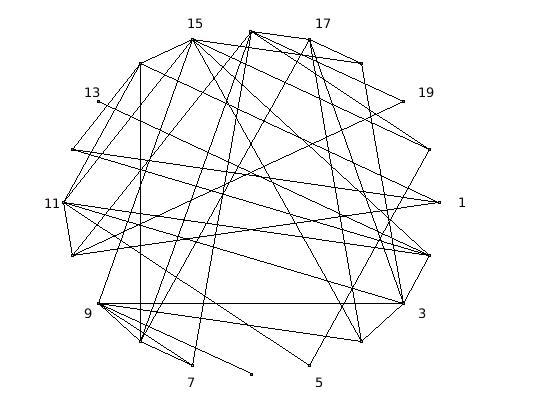
\includegraphics[width=\textwidth]{Graphs/P0_9_Network.jpg}
		\caption{Representation of Strogatz network with p=0. Every line represents a connection between the two linked nodes. A regular grid is formed.}
		\label{fig:regular_network}
	\end{minipage}
	\hfill
		\begin{minipage}[c]{0.45\textwidth}
			\centering
			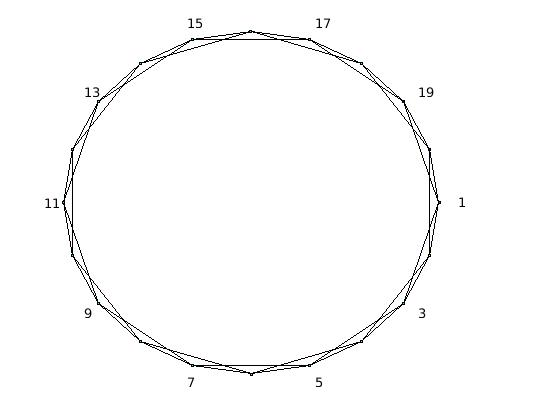
\includegraphics[width=\textwidth]{Graphs/Regular_Network.jpg}
			\caption{Representation of Strogatz network with p=0.9. Every line represents a connection between the two linked nodes. A random grid is formed.}
			\label{fig:random_network}
		\end{minipage}
\end{figure}

The input parameters are the network size, the probability of rewiring a contact and the mean number of friends per agent. After rewiring certain connections the agents will have a chance to not build any friendships. This issue is resolved by forming a connection to a randomly chosen node for all agents that do not have at least one friend. This step is required to not change the outcome of the later simulation process in an unrealistic way. Also the existing code had to be adapted such that a friendship cannot be formed between the agent and himself.

The information of the friendship distributions in the network are stored in upper triangular matrices. For simplicity the two upper triangular matrices of the real-life and Facebook\textsuperscript{\textregistered} networks are merged for the simulation (see fig. \ref{fig:Matrix}).
\begin{figure}
	\centering
	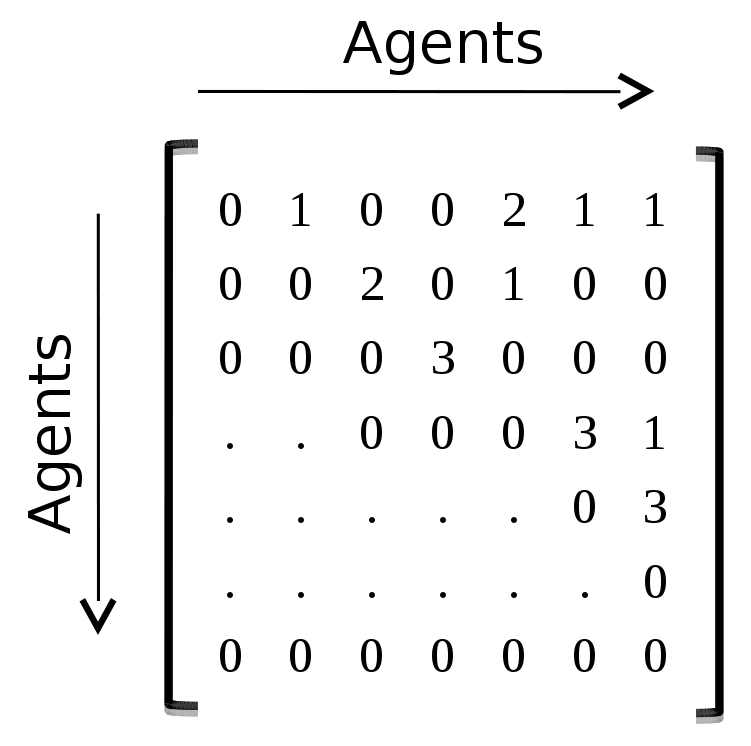
\includegraphics[width=0.4\textwidth]{Graphs/Matrix2.png}
	\caption{Upper triangular matrix for agents network. The values 1 depict a social network friendship whereas 2 denotes a close friendship, 3 accordingly means both.}
	\label{fig:Matrix}
\end{figure}

\subsection{Simulation}
During the investigation on how to influence a social system in the most efficient way the network has to be fixed, such that the randomness of the network generation will not affect the outcome.

After that is made sure a certain number of agents will be influenced. According to the lead question of this work, a limited budget is available. This means only a limited number of agents can be influenced. Throughout the simulation this “target group” cannot be changed anymore. The number of agents to be influenced was chosen to be 3\%, 8\% or 10\% of the total number of agents available in the system. 

The target group was defined by the degree of connectivity of the agents (number of friendships). 
\\ 

The three groups were:

\begin{itemize}
\item The agents with the highest connectivity
\item The agents with the lowest connectivity
\item The agents with exactly the mean number of friendships of the underlying system
\end{itemize}

More weight was given to close friendships than to social system friendships by saying 1 close friendship is equivalent to 2 social system friendships. 

To make a statement about the “effectiveness” of the information spread the number of iterations necessary to reach a certain overall opinion threshold (eg. -0.9) was determined. 

To compare the speed of reaching this threshold for different simulation parameters, a “benchmark time” is necessary. It is found when simulating the opinion development a 1000 times, while choosing random agents to be influenced. For every iteration the number of simulations, that is necessary for an averaged opinion of all agents to reach the value -0.9,  is chosen.

This results in 1000 simulation number, that are averaged to get the benchmark time. 

The simulation loops through all agents and adapts their opinion, based on the opinions of their friends. Normally this is done by averaging the opinion of all of their friends with different weighting for real-life and social network friends. The new opinion of the current agent is then then determined by changing the old opinion up to a certain percentage, that is based on the gullibility of the current agent, with the described average opinion of their friends.

\begin{equation*}
x_{new} = (1-g) * x_{current} + g * (k_{FB} *x_{FB} + k_{CF} * x_{CF}) / (k_{FB} +n_{FB} +k_{CF} *n_{CF})
\end{equation*}



$x_{new}$ and $x_{current}$ stand for the agents new respectively current opinion. g is the gullibility of the agent and the constants nFB, nCF are the number of social media friends respectively close friends that agent has. $k_{FB}$ and $k_{CF}$ are constants that put more weight to close friends than social media friends.  

The new opinion is then stored in a temporal variable in order to allow the other agents to form their opinion based on the old opinion of the all other agents.

If an agent is influenced however the opinion formation formula has to be adapted. These agents do not change their own opinion (it is fixed at -1).

After the new opinions of all agents are formed, the old opinions of the agents will be updated at the same time and the loop continues.


To find what influencing model is most efficient, one can look the rate of opinion changing. The longer it takes for the agents to reach the threshold opinion, which is close to that of the influencer, the less efficient the influencing was.


\section{Simulation Results and Discussion}

In this section, we present our experimental evaluation on synthetic data. Our results on synthetically generated data show that the main factor for spreading information is the amount of people that are initially convinced. We suppose it is not cost efficient to search the top-connected agents in a new random network. At some point it becomes more economical to invest in randomly chosen agents than to invest in research to find the best-connected agents. Our results show that the time needed to convince 90\% by choosing the best-connected agents compared with choosing random agents is around 50\% slower if we go for the randomly chosen agents. A much better approach for reducing the time to convince 90\% is by increasing the number of initial agents that are convinced by the given information.

\subsection{Dataset and Implementation}

The network we implemented is based on the Strogatz model which is used for generating random graphs. In our case, we need a network representing the social life of a human being. To keep it simple we reduce the social interaction into two groups: close friends and social media friends. For simplicity reasons social media friends will be referred to as Facebook\textsuperscript{\textregistered} friends.

A random graph represents our network. Truly generated graphs should have a Gaussian distribution of number of Facebook\textsuperscript{\textregistered} friends as well as number of close friends. Plotting both distributions should confirm that the network was randomly generated.

\subsection{Analyzing the Friendship Network}

\begin{figure}
	\centering
	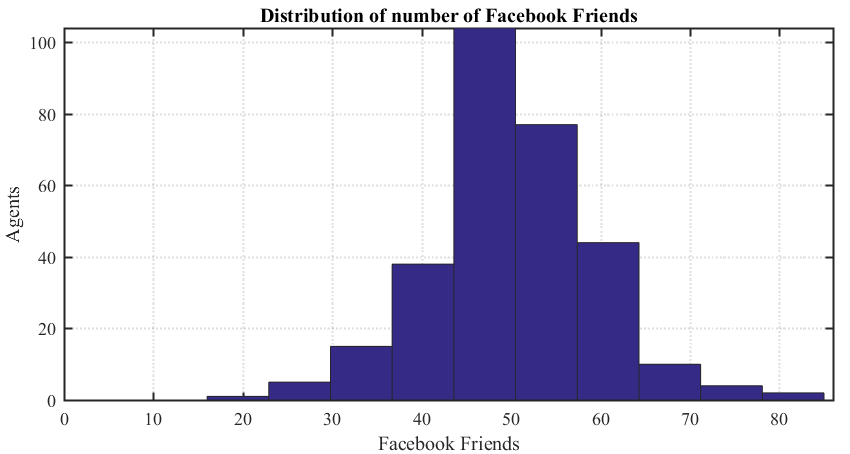
\includegraphics[width=\textwidth]{Graphs/Dist_FB.png}
	\caption{The distribution of Facebook\textsuperscript{\textregistered} friends follows a Gaussian distribution.}
	\label{fig:DistFB}
\end{figure}

As can be seen in fig. \ref{fig:DistFB}, the randomly generated network has a Gaussian distribution with an expected value of approximately 48 Facebook\textsuperscript{\textregistered} friends per agent.

\begin{figure}
	\centering
	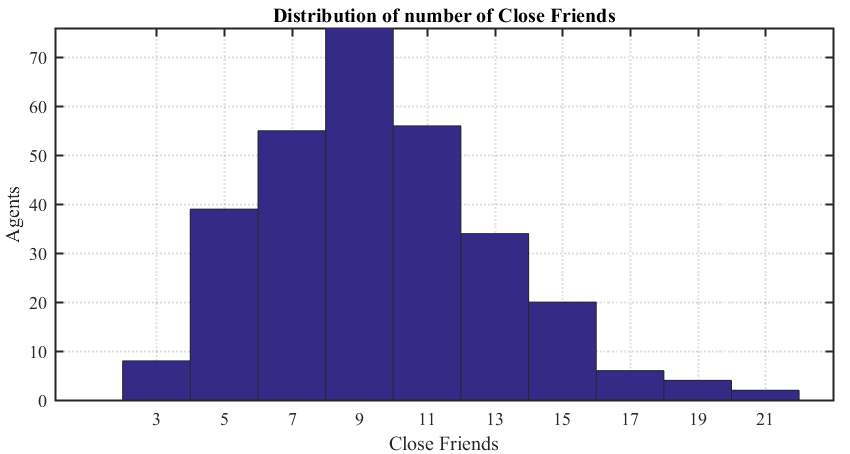
\includegraphics[width=\textwidth]{Graphs/Dist_CF.png}
	\caption{The distribution of close friends also follows a Gaussian distribution.}
	\label{fig:DistCF}
\end{figure}

As fig. \ref{fig:DistCF} shows, the randomly generated network has a Gaussian distribution with an expected value of approximately 9 close friends per agent.

\textbf{Important:} for all calculations the same Network was used!

\subsection{Influencing Different Initial Groups}
We compare the three different outcomes. For each, a group of agents that were influenced in the beginning and have set their opinion to -1 have to be chosen. We compare the change of the average opinion for the following three groups: Group 1, choosing the best connected Agents in the Network as the initially influenced persons, Group 2, choosing random Agents, and Group 3, choosing the Agents with the least friends. As expected, it is most efficient when initially influencing the best connected agents. We want to investigate how cost efficient it is to search for the best connected agents in a network, compared with investing in more initial influenced agents that are chosen randomly. As point of reference, we also calculated the worst case scenario, meaning, having chosen the least connected agents.

\subsection{Analyzing the Opinion Data}

The plots consist of 4 graphs: “Worst connected agents” represent the average opinion development over time if the least connected agents were chosen. “Average connected agents” stand for the randomly chosen Agents. Because this varies according to the randomness, thousand different outcomes for choosing random agents we calculated and the mean value of all those outcomes will be referred to as the average connected agents. The best connected agents are represented as well in the plot. As point of reverence, we also plotted the value -0.9, which helps visualize the point in time when the average opinion dropped below this value.

The different plots represent the different percentages of initially influenced agents. For all calculations, the same randomly generated Network was used.

\begin{figure}
	\centering
	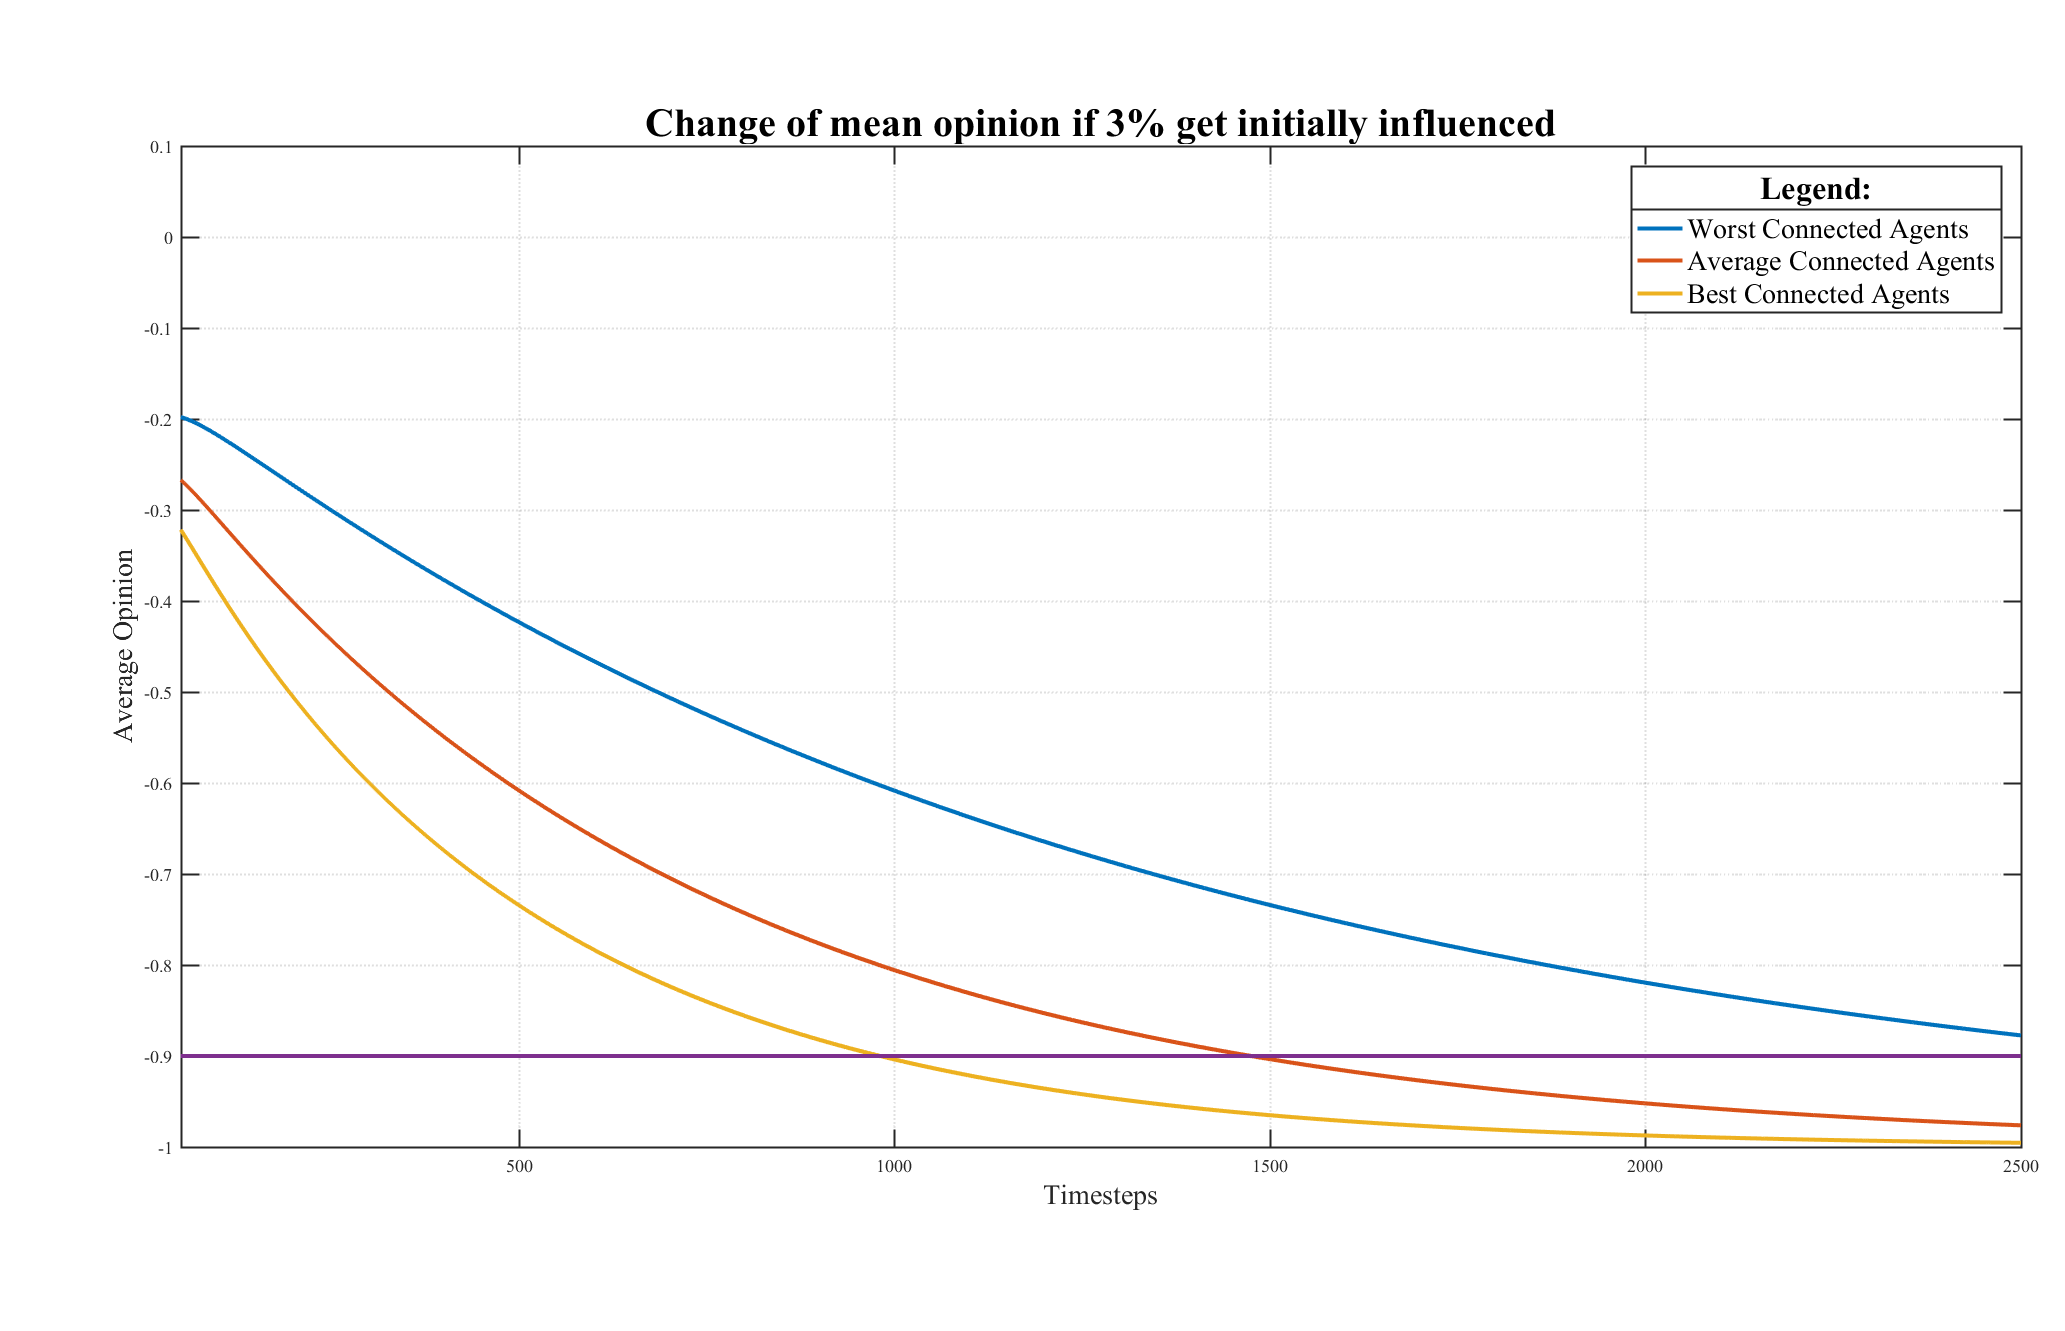
\includegraphics[width=\textwidth]{Graphs/3percent.png}
	\caption{Influencing 3\% of all existing agents one can see that the opinion drops rather slowly.}
	\label{fig:plot3}
\end{figure}

Influencing the top three percent connected agents the average opinion will drop below -0.9 after approximately 1000 timesteps. Choosing random agents, this process will take 50\% more time. The worst Case scenario is almost three times longer (see fig. \ref{fig:plot3}).

\begin{figure}
	\centering
	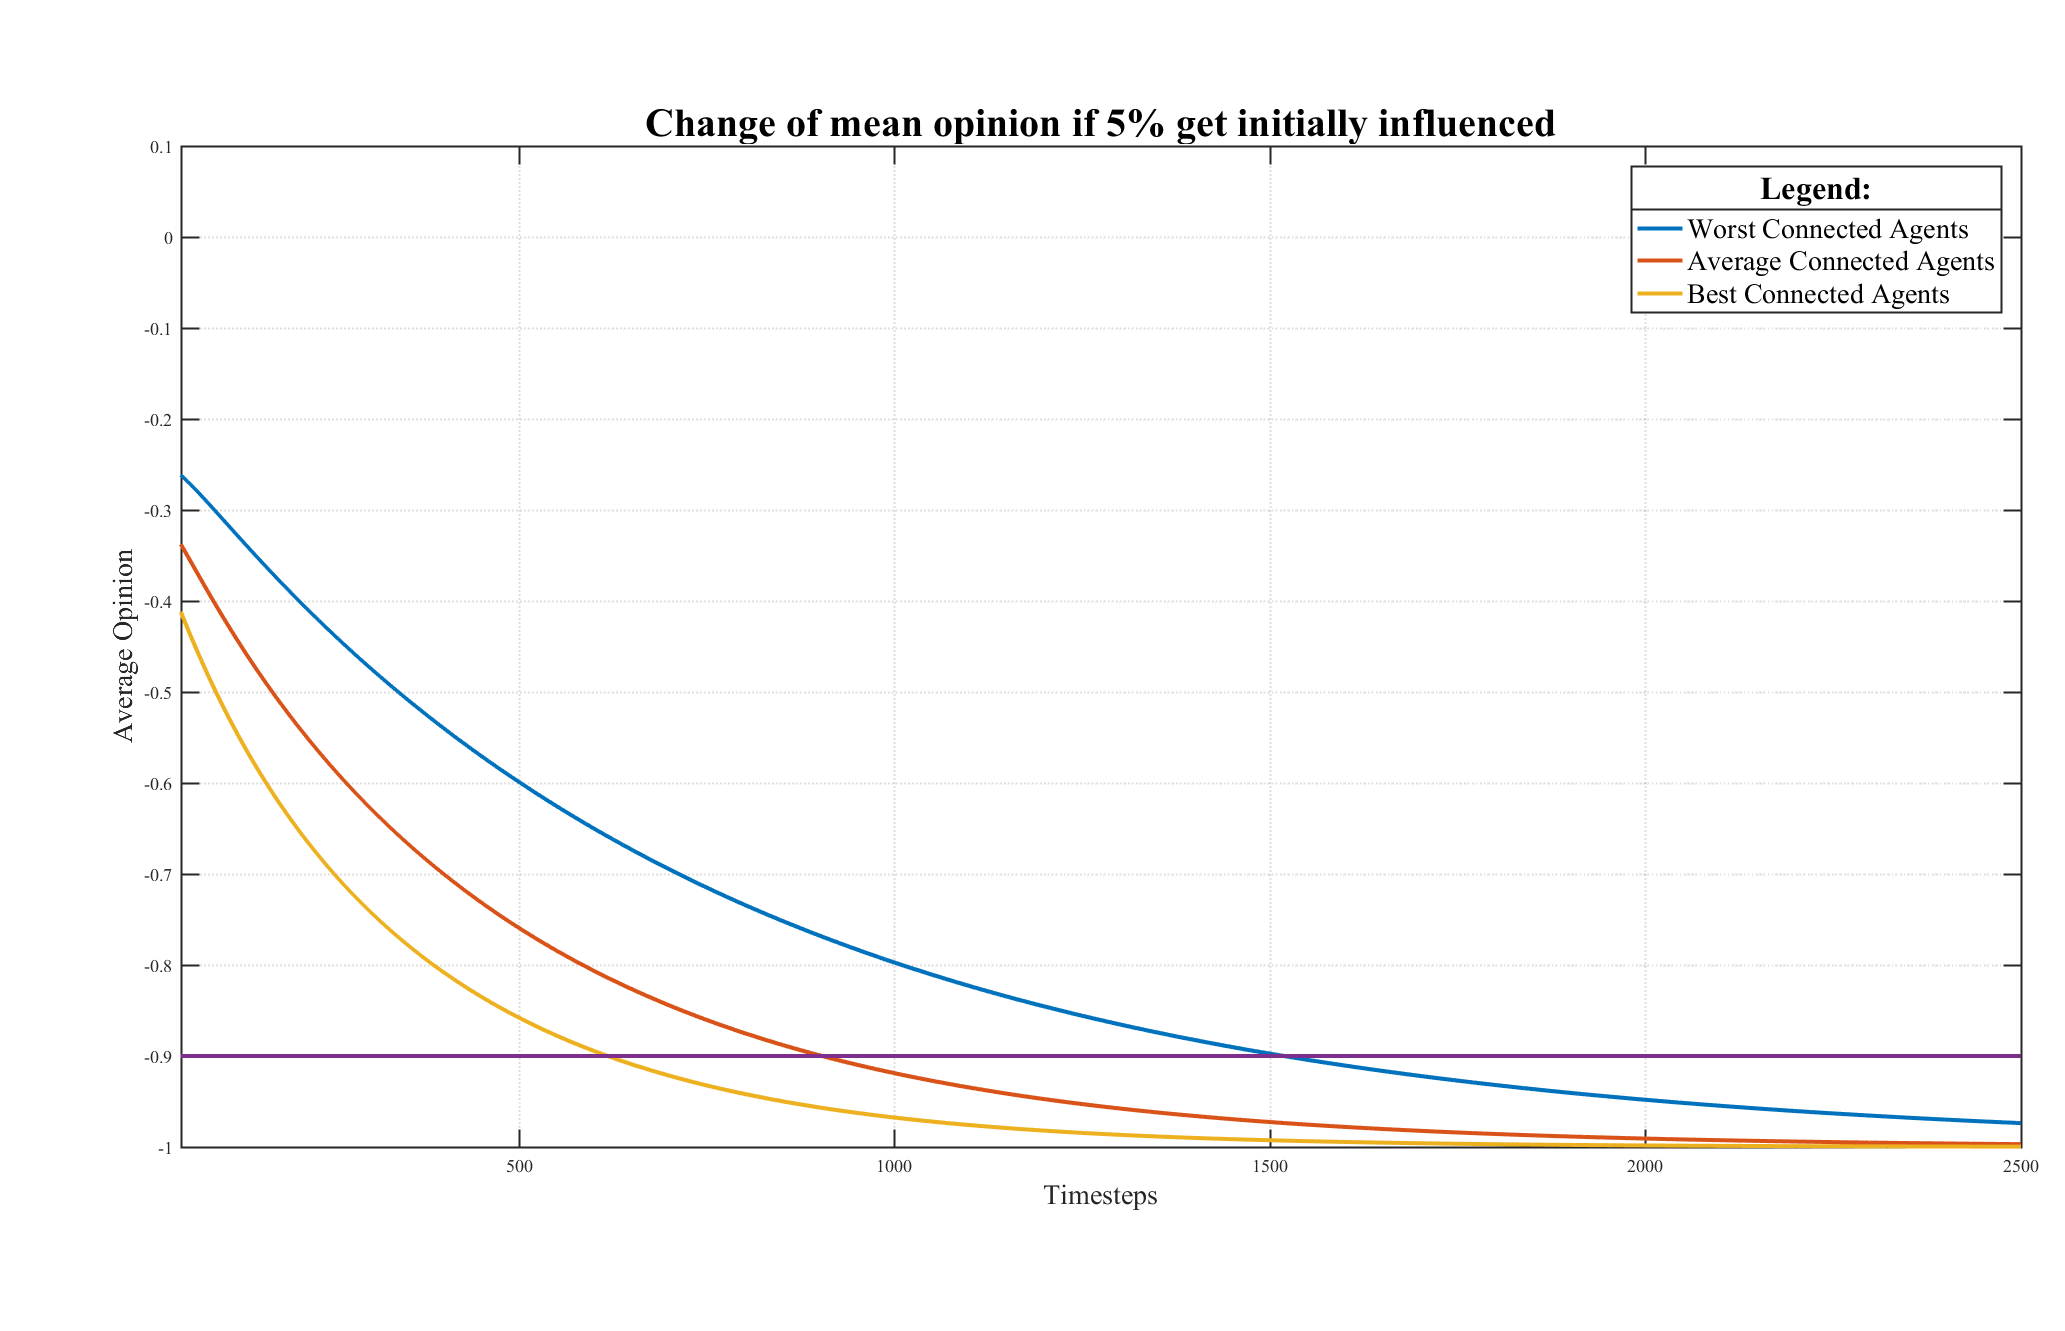
\includegraphics[width=\textwidth]{Graphs/5percent.png}
	\caption{Influencing 5\% of all existing agents one can see that the opinion drops overall opinion drops faster.}
	\label{fig:plot5}
\end{figure}

Influencing only two percent more agents, the average opinion will drop a lot faster. Interestingly, the average opinion of the randomly chosen agents reaches the reference point earlier than if one were to investigate the network for the best three connected percent of agents and influence them. This worst case scenario is as good as if three instead of five percent of random agents were chosen (see fig. \ref{fig:plot5}).

\begin{figure}
	\centering
	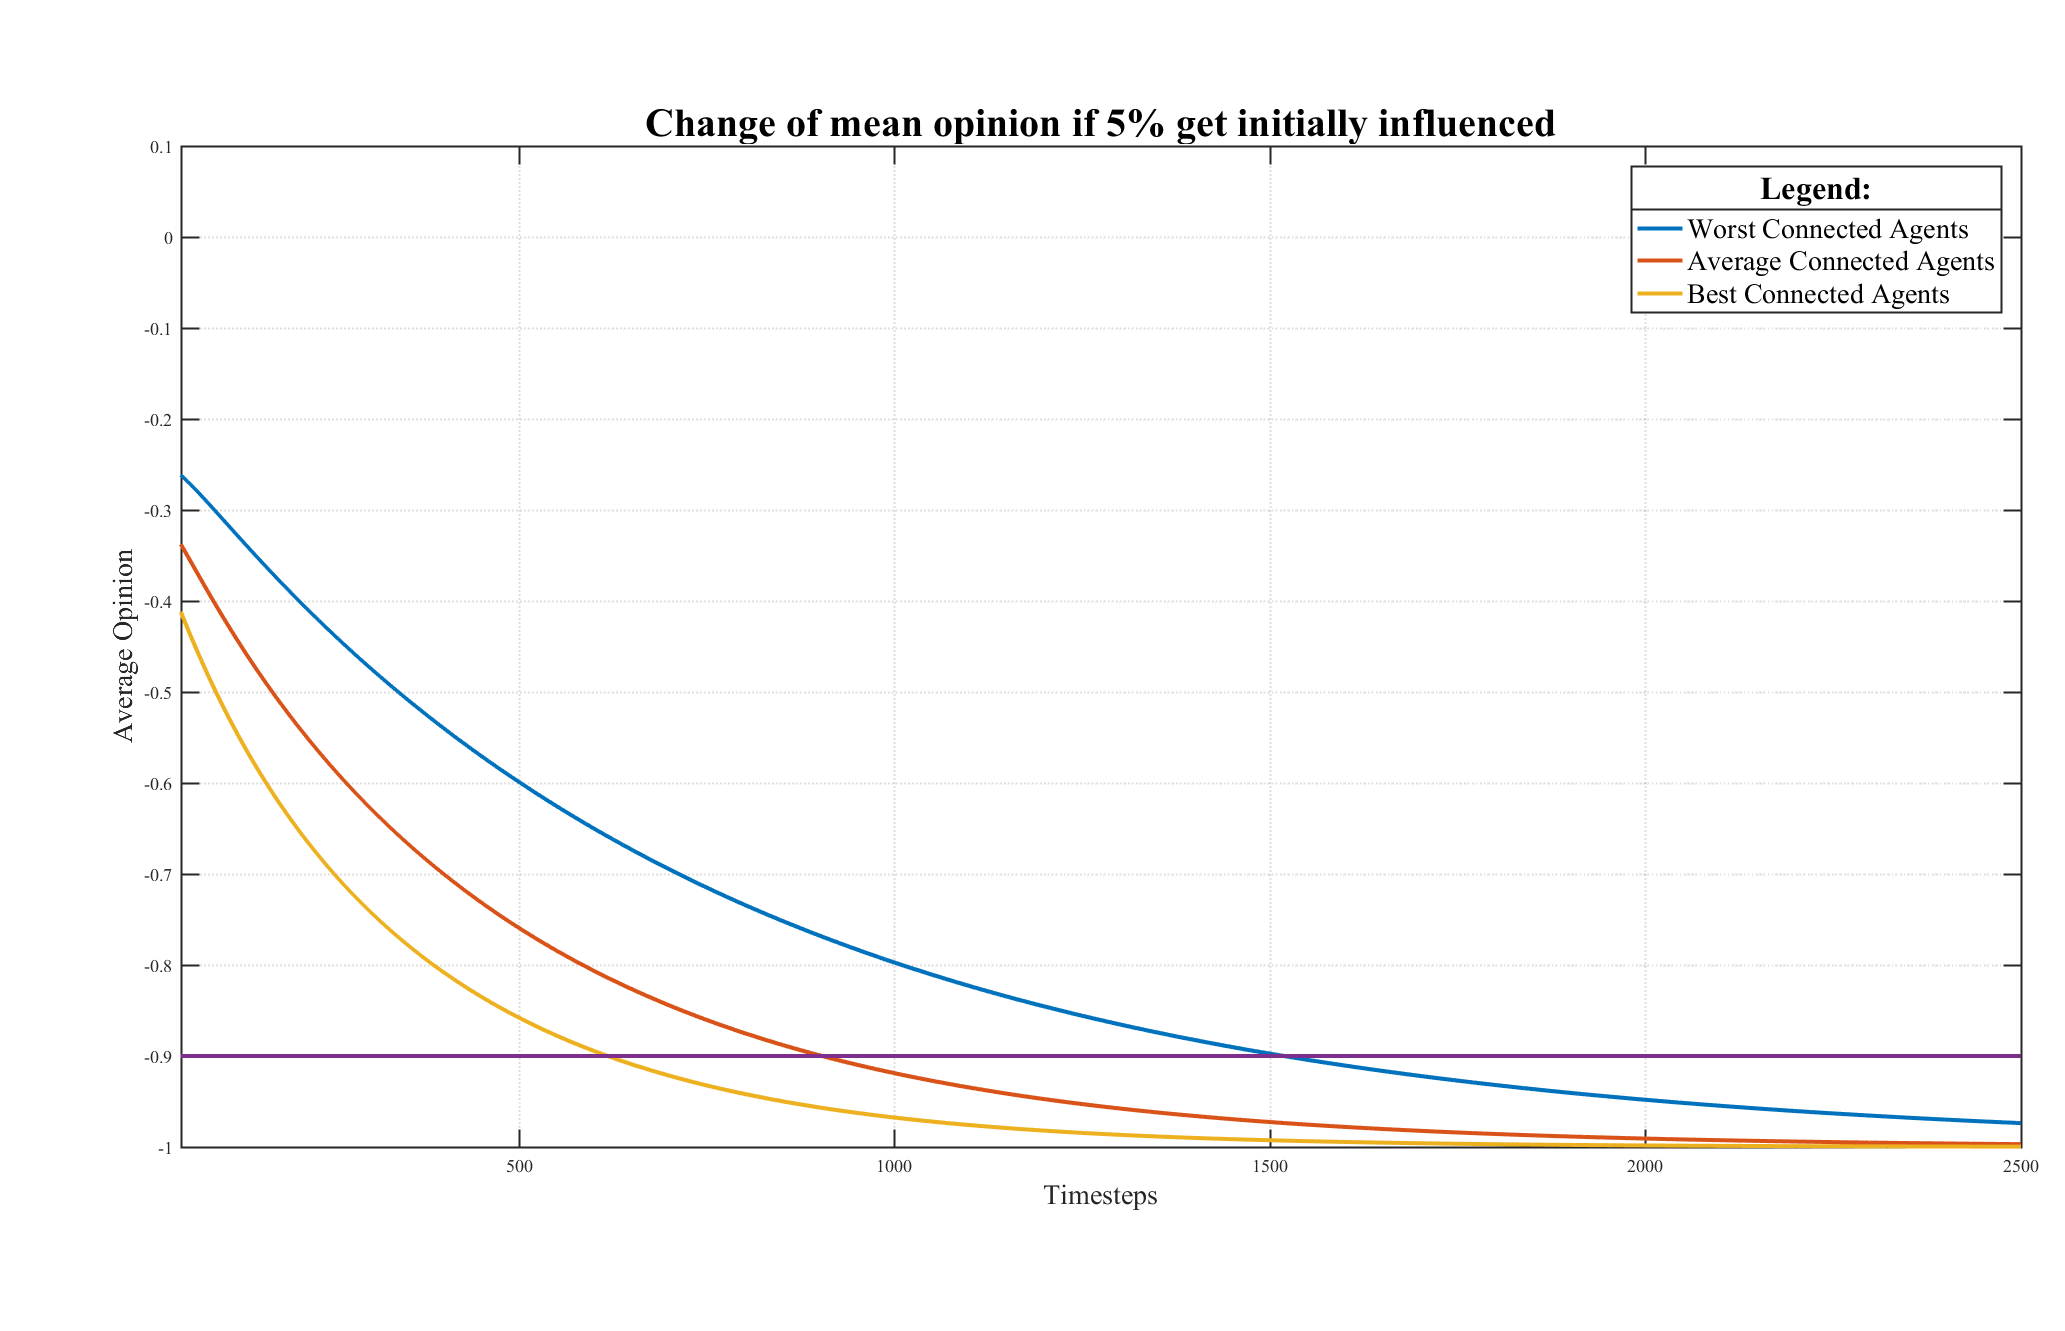
\includegraphics[width=\textwidth]{Graphs/5percent.png}
	\caption{Influencing 8\% leads to an increasingly negative slope of all graphs.}
	\label{fig:plot8}
\end{figure}

Adding another three percent will again improve the average connected agents so that they can be compared to the best five percent connected agents. The last two plots show, that increasing the percentage will continuously improve but it needs to be considered that more Initial influenced agents will be costlier as well (see fig. \ref{fig:plot8},\ref{fig:plot10}).

\begin{figure}
	\centering
	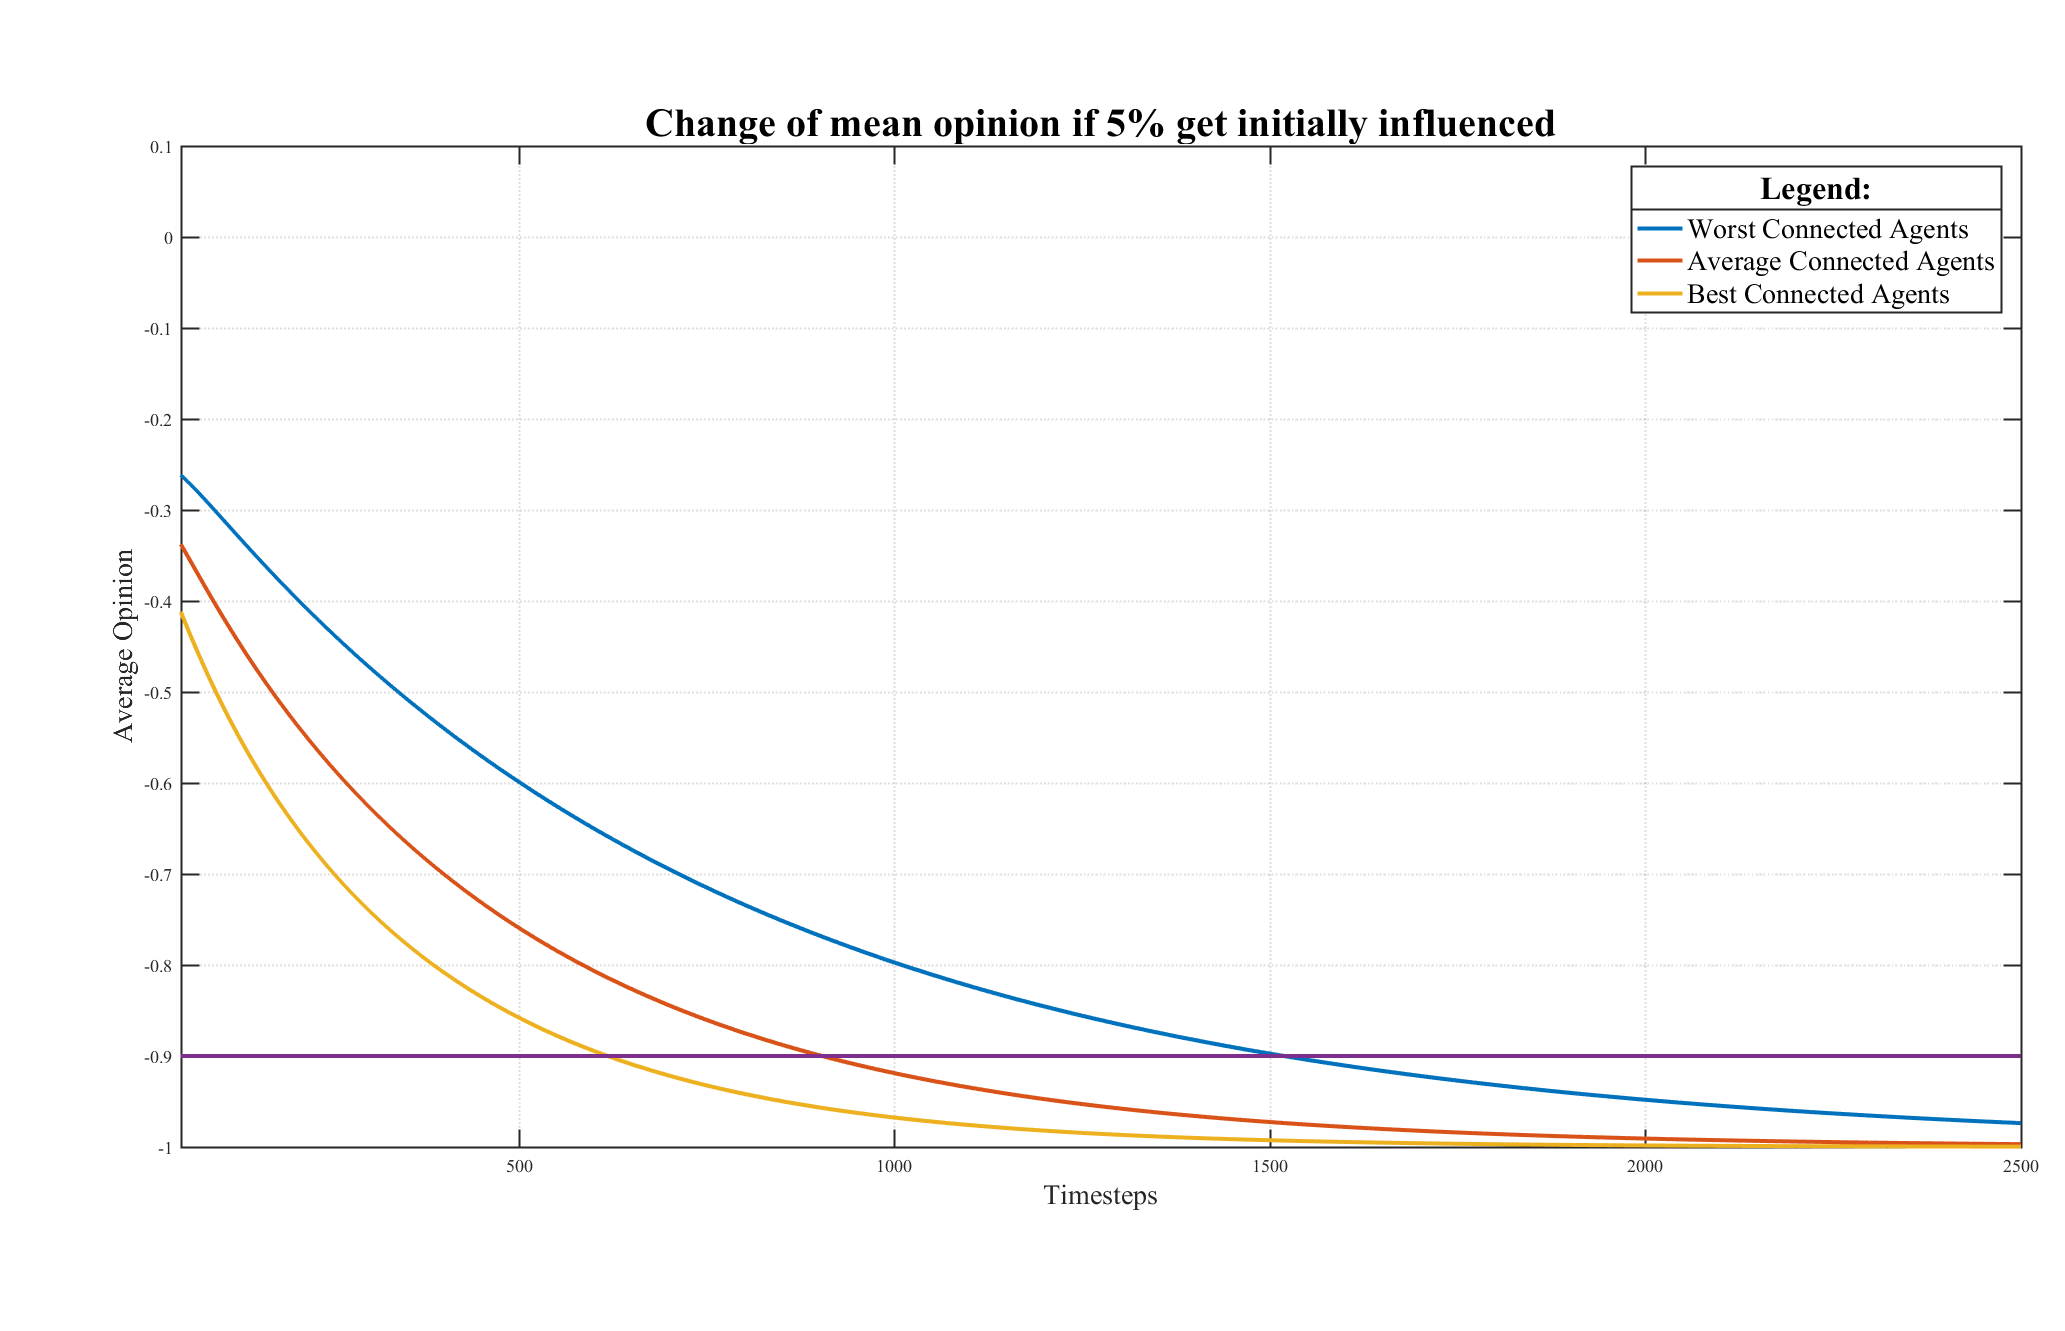
\includegraphics[width=\textwidth]{Graphs/5percent.png}
	\caption{Influencing 10\% leads once more to a faster change in opinion. It is especially beneficial for the average and worst connected agents.}
	\label{fig:plot10}
\end{figure}

All plots represent the mean value of all the agents in the network. The results show that influencing five percent of all agents by randomly choosing them is as good as investing in searching for the top three percent of agents. From this simulation it is clear that product or information placement should be spread on a wider range rather than focusing too much in searching the best placement, in a condition that one has the budget to do so. 


\section{Summary and Outlook}

In conclusion, we have shown that in conditions of restricted budget the target individuals subject to initial information placement have to be carefully chosen. As a matter of fact the choice of agents with highest social capital (largest number of friends) leads to a significant decrease in time that takes the information become viral. On the other hand, we showed, that in a condition when the budget restriction is waived, the best strategy is to target a large pool of individuals without searching for those with highest social impact among their peers, as this yields the same pace of information spread without requiring additional efforts of picking the initial agents.   
\section{References}

\begingroup
\renewcommand{\section}[2]{ }

\begin{thebibliography}{9}
	\bibitem{NHB1}
	Xiaoyan Qiu et al,
	\textit{Limited individual attention and online virality of low-quality information},
	Nature Human Behaviour 1,
	Article number: 0132,
	2017.
	
	\bibitem{Network1}
	Pablo Blinder, \textit{https://ch.mathworks.com/matlabcentral/fileexchange/4206-erdos-renyi-random-graph}, (State of 09.12.17)
	
	\bibitem{Network2}
	Duncan J. Watts \& Steven H. Strogatz,
	\textit{Collective dynamics of ‘small-world’ networks},
	Nature,
	1998.
	
\end{thebibliography}
\endgroup

\newpage
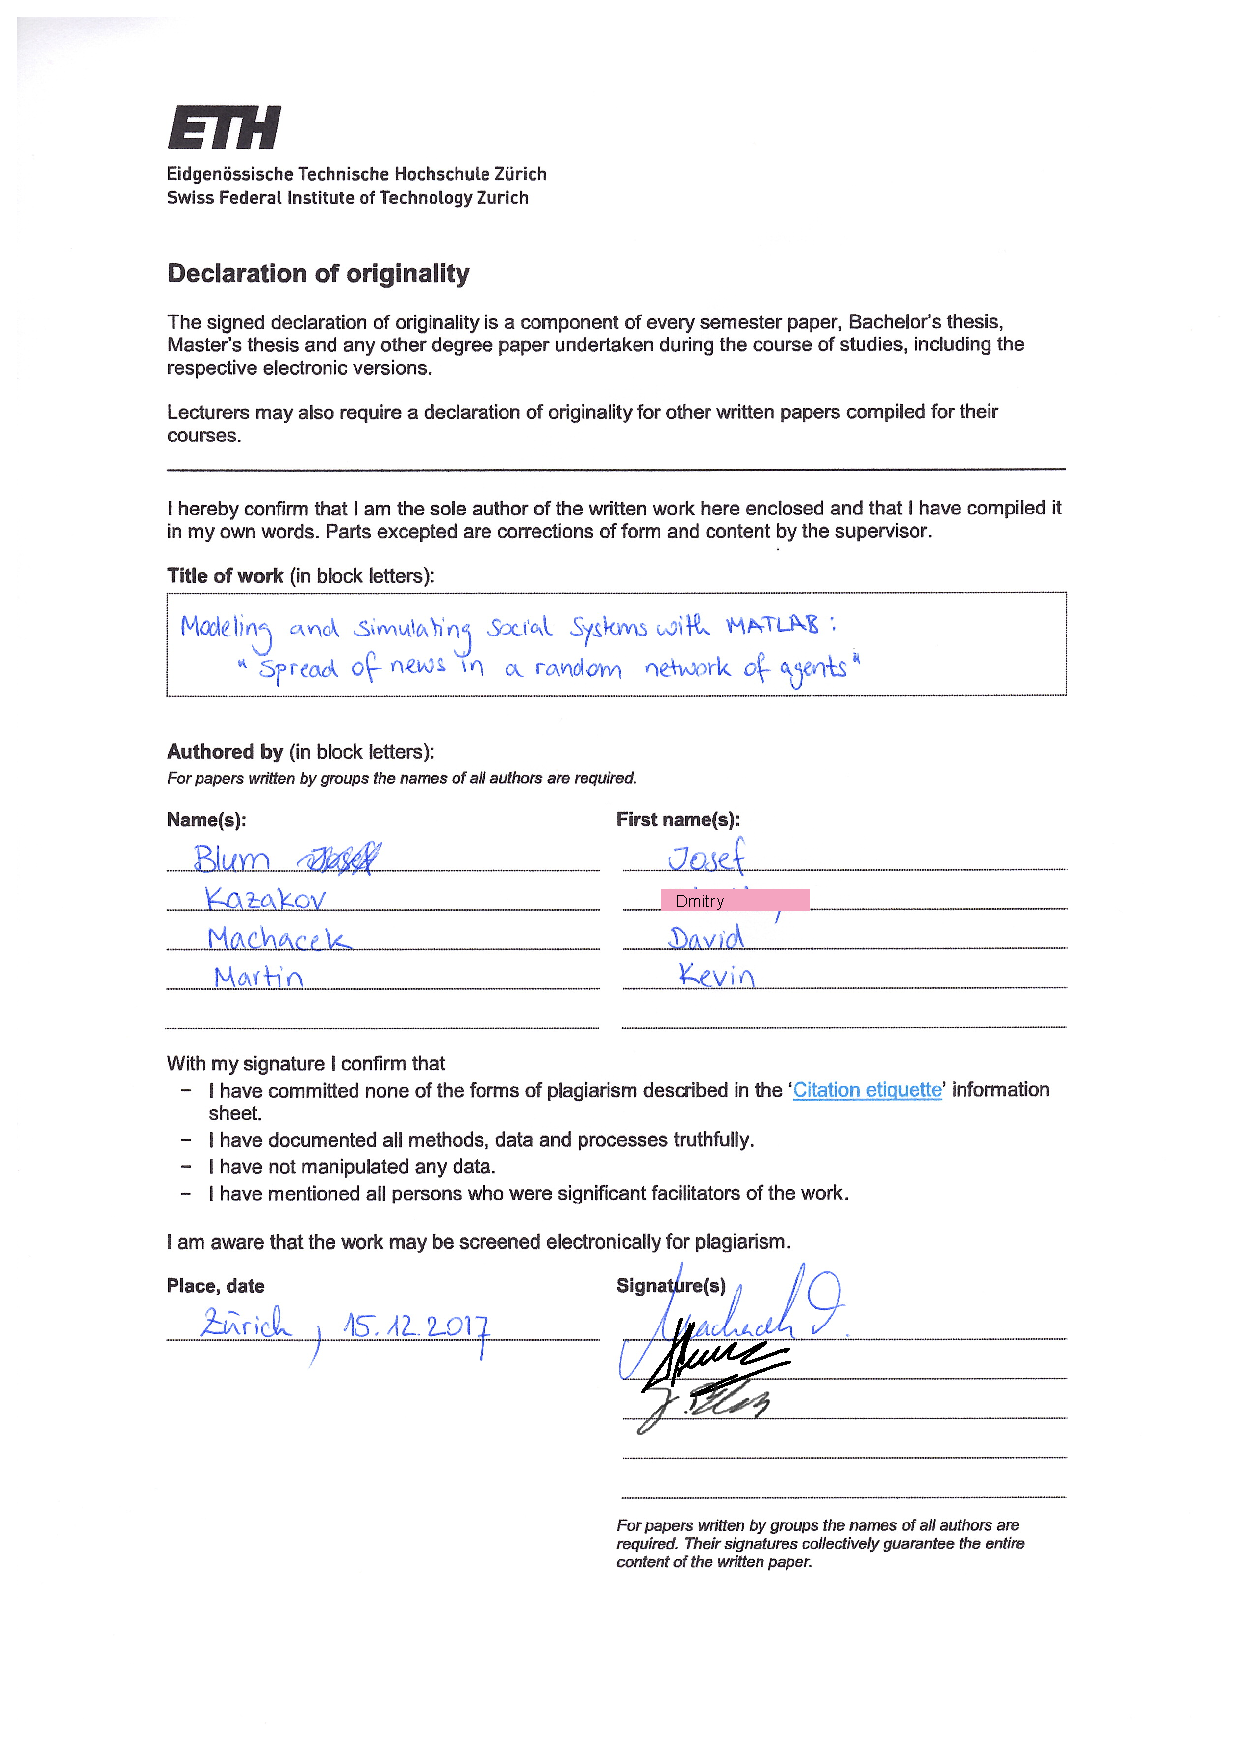
\includepdf[fitpaper=true, pages=-]{Graphs/DecOrginiality.pdf}

\end{document}  



 
